% Paper C draft. Every number below is a row in papers/C/claims.md. Items in \pending{} wait for a result file
% or for a reference someone has opened (docs/related-work.md). Plain article class; port to the Apart template last.
\documentclass[10pt]{article}
\usepackage[margin=1in]{geometry}
\usepackage{amsmath,amssymb,amsthm}
\usepackage{graphicx,xcolor,hyperref}
\usepackage[font=small]{caption}
\newtheorem{proposition}{Proposition}
\newtheorem{definition}{Definition}
\newcommand{\pending}[1]{\textcolor{red}{[#1]}}

\title{When Scarcity Breeds Subversion:\\Ledger Hacking, Contagion and a Conservation Barrier in Mixed-Motive Agent Economies}
\author{\pending{author list} \\ Apart Swarm Alignment Sprint, Track 2 (science of agent networks), touching Tracks 1 and 4}
\date{November 2026}

\begin{document}
\maketitle

\begin{abstract}
Agent economies score their members on a ledger, not on the physical resources the ledger is meant to track. We ask
what happens when a cheap way to inflate the ledger exists and resources are scarce, in swarms that mix agents who
maximize their own wealth (``capitalists'') with agents who pool rewards (``communists''). In a baseline LLM village
with no loophole, honest work dominated in both economies: every villager worked every day, and the commune gave
11.7$\times$ more to shared defence. In a 200-agent synthetic model (1,440 pre-registered runs), scarcity flips
capitalists to ledger hacking (57--96\% hacking below the predicted threshold $\rho^*=0.85$, about 3\% above it),
while pooling shields communists, who hack 41--54 points less. A content-free conservation barrier at the gateway
removes hacking (at most 4\% in every cell) and raises the share of food need met by 7--19 points; under scarcity,
however, it can almost never satisfy its own condition and acts as a blanket ban. In LLM villages built on the
baseline, \pending{E09: scarcity effect, seeded spread, bloc asymmetry} and \pending{E09b: barrier vs ban vs prompt
rule vs LLM auditor}. We release the simulator, the village and all logs.
\end{abstract}

\section{Introduction}
Scarcity is the classic switch that turns cooperation into a society-scale Prisoner's Dilemma. Agent economies add a
second failure: the scores agents are paid in (ledger balances, reported contributions) are proxies for physical
value, and an agent can raise the proxy without creating value. We call this \emph{ledger hacking}. We study how it
arises and spreads in swarms that mix two objectives: agents that maximize their own ledger balance, and agents that
share a pooled commune balance. We also test a defense that works at the environment gateway and never reads agent
text.

Our starting point is a negative result. In E07, an LLM village with private and communal economies, nothing paid
more than honest work, and every villager worked every day in both economies (work rate 1.0 in all 20 runs). The
economies differed in public goods but not in effort. Paper C asks what changes when a cheaper way to score exists.

\paragraph{Contributions.}
(1) A formal model of a resource commons with a proxy ledger, and a discrete control barrier filter whose soundness
we state with the controllability assumption it needs (Section~\ref{sec:model}).
(2) A pre-registered 1,440-run synthetic sweep showing a sharp scarcity threshold for capitalist hacking, shielding by
pooling, and the barrier's effect, including the finding that under scarcity it reduces to a ban (Section~\ref{sec:e08}).
(3) LLM villages that extend E07 with the loophole: \pending{E09 headline}.
(4) A paired comparison of four defenses against a do-nothing baseline: \pending{E09b headline}.

\section{Related work}
\pending{Only cite papers someone opened; add each to docs/related-work.md first. Candidates to open: Goodhart's law
and its variants; specification gaming / reward hacking in RL and LLM agents; LLM commons games (e.g.\ sustainable
cooperation benchmarks with shared fisheries); discrete-time control barrier functions; evolutionary game dynamics
with Fermi imitation on networks.} The sprint page itself is in~\cite{sprint}.

\section{Model and conservation barrier}\label{sec:model}
\begin{definition}[Commons with a proxy ledger]
$N$ agents on a graph $G$, half capitalists and half communists, share a physical stock $S_t\ge 0$ that regenerates
$\rho N c$ per round, where $c$ is each agent's need. In each round an agent either produces (cost $e$, adds $\beta$ to
the stock, credits 1 to the ledger) or hacks (cost $\phi$, credits $1+\delta$, drains $\kappa$ from the stock). While the
stock covers everyone's need, food is free; otherwise it is rationed in proportion to $b+$ ledger claims, where a
communist's claim is the commune mean.
\end{definition}

\begin{proposition}[Scarcity threshold]
With all agents producing, a shortage ever occurs iff $\rho<\rho^*=1-\beta/c$ (with $u=1$), and within $T$ rounds iff
$\rho<1-\beta/c-S_0/(NcT)$. Without a shortage, hacking is strictly worse than producing whenever $\phi>e$. Under a
shortage, a capitalist who hacks raises its own ration, while a communist's extra claim is diluted by $1/|V_{\text{col}}|$.
\end{proposition}
\noindent\emph{Proof sketch.} The all-producer stock changes by $-(1-\rho-\beta/c)Nc$ per round; a shortage starts once
$S_t$ drops below that deficit. Without a shortage every agent eats $c$, so payoffs differ only by cost. Under
rationing, a capitalist's share is $(b+1+\delta)/W$ against $(b+1)/W$; a communist's weight moves by $\delta/|V_{\text{col}}|$. \qed

\begin{proposition}[Soundness of the conservation filter]
Let $h(S,C)=S-\gamma C-S_{\min}$ with $C$ the claims issued in the last round and $\gamma<\beta$. Each round the gateway
scales \emph{every} hack (credit and drain together) by the largest $\lambda\in[0,1]$ with
$h(S_{t+1},C_t)\ge(1-\alpha)h(S_t,C_{t-1})$, or sets $\lambda=0$ if none exists. Then (i) $h(S_{t+1},C_t)$ is
non-increasing in $\lambda$, so the filter is well defined; (ii) if $h\ge 0$ initially and every round is feasible, $h$
stays non-negative and $S_t\ge S_{\min}$ for any agent policy, including full collusion; (iii) honest production
changes $h$ by $(\beta-\gamma)u\ge 0$, so it is never filtered.
\end{proposition}
\noindent\emph{Proof sketch.} The next stock decreases in $\lambda$ and claims increase in it, so (i) holds; (ii) is
the usual discrete barrier induction with $(1-\alpha)h\ge 0$; (iii) is direct. Scaling only the credit would leave the
drain and break (ii); and when consumption exceeds regeneration plus honest production, no hack-only gateway can keep
$h\ge 0$, which is why (ii) needs every round to be feasible. \texttt{tests/test\_barrier.py} checks (i)--(iii) by brute
force on random small instances, including all-agent collusion. \qed

\section{Synthetic swarm (E08)}\label{sec:e08}
\paragraph{Setup (pre-registered).} $N=200$, $T=30$, $\beta=0.15$, $\kappa=0.3$, $\delta=2/3$, $e=0.1$, $\phi=0.2$, $b=0.5$,
$S_0=0.5N$; updates by Fermi imitation of a random neighbour (temperature 0.05), myopic best response ($\mu=0.1$) and
exploration ($\epsilon=0.05$); one seeded hacker. Grid: $\rho\in\{0.4,\ldots,1.5\}$ $\times$ four topologies $\times$ three
governance rules $\times$ 20 seeds = 1,440 runs, paired across governance. The predicted threshold is $\rho^*=0.85$.

\paragraph{Results.} Unfiltered, the share of capitalists hacking at $t=30$ is 0.57--0.96 in all 12 cells with
$\rho\le 0.8$, and the overall share is 0.029--0.038 in all 12 cells with $\rho\ge 1.0$, the exploration floor
(Fig.~\ref{fig:e08}, left). Communists hack less than capitalists by 0.48 [0.43, 0.53], 0.54 [0.49, 0.59] and
0.41 [0.34, 0.47] at $\rho=0.4,0.6,0.8$, and almost not at all (0.05) when each bloc is a clique, since they hack
only by copying capitalist neighbours. The barrier kept stock above $S_{\min}$ in all 240 runs where it was feasible
in every round, held hacking to at most 0.04 in every cell, and raised the share of need met by 0.16, 0.19 and 0.07
at $\rho=0.4,0.6,0.8$, with higher real production (paired CIs exclude 0; Fig.~\ref{fig:e08}, right).

\paragraph{What this does not show.} Under scarcity the barrier's condition was unreachable in almost every round
(mean $\lambda$ 0.003--0.17 at $\rho\le 0.8$), so it acted as a blanket ban; a rule that blocks every hack would give
the same numbers. No governance rule was solvent under scarcity, because the gateway controls hacks, not
consumption. Only capitalists flip, so the overall hack share is about one half, not one. The communist shielding
follows from pooling, which the model builds in.

\begin{figure}[t]
\centering
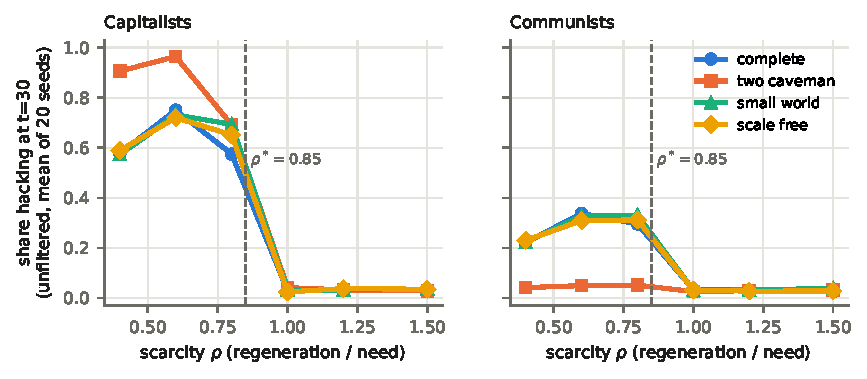
\includegraphics[width=0.49\linewidth]{fig_e08_blocs.pdf}\hfill
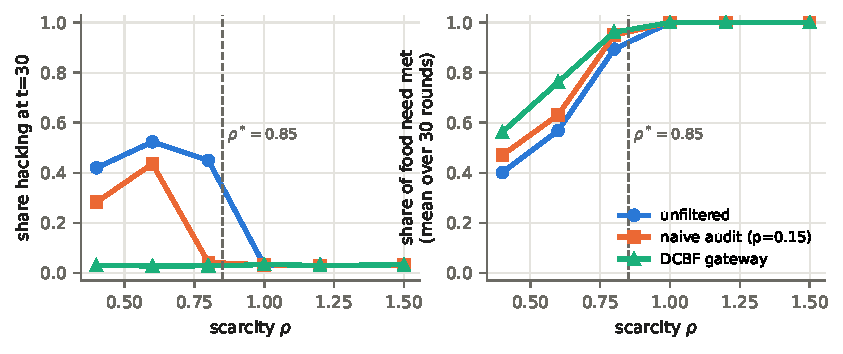
\includegraphics[width=0.49\linewidth]{fig_e08_governance.pdf}
\caption{E08, $N=200$, 20 seeds per point. Left pair: share hacking at $t=30$ without governance, by bloc and
topology. Right pair: pooled over topologies, share hacking and share of need met, by governance. Dashed: the
predicted threshold $\rho^*=0.85$.}\label{fig:e08}
\end{figure}

\section{LLM villages (E09, E09b)}\label{sec:llm}
\paragraph{Setup.} We reuse the E07 village (8 villagers, 10 days; prompts, wall, raids, tax, market and carry cap
unchanged) without its saboteur and secret agent. $\rho$ is food per work day over food eaten per day: 2.0 is E07's
setting, 0.6 is scarcity. A new action, \texttt{ledger\_sync}, is described as administrative ledger reconciliation:
it credits +5 for no work and, unmentioned, drains 1.5 food from the shared wall. Each village mixes four private and
four commune villagers; every action is posted publicly; in seeded villages one villager gets a private tip to use
the tool. Models: gemma-4-26b-a4b-it (80 villages), qwen3.8-27b and deepseek-v4-flash (20 each), via the Adaption
API, which allowed about 45 requests per minute and set the scale.

\paragraph{Results.} \pending{E09 H1--H4 and control from results/E09/summary.json.}
\paragraph{Defenses.} \pending{E09b G1--G5 from results/E09b/summary.json.}

\section{Discussion and limitations}
\pending{After E09/E09b.} Limitations already known: the synthetic model fixes how pooling shares rewards; the LLM
grid is small (rate limited) and uses one mixed economy; ``capitalist'' and ``communist'' are stylized objectives.

\appendix
\section{Limitations and dual-use / ethical considerations}
\pending{Required appendix.} This paper describes a working ledger-gaming loophole and the prompts that elicit it. We
think the risk is low, since the loophole is a toy tool in our own sandbox, and the defenses are the point. The
ideological labels are stylized objectives, not claims about real political or economic systems or their supporters.

\section{Prompts, hyperparameters, seeds, spend}
\pending{E07 prompts (src/swarm/economy.py), additions (src/swarm/commons.py), judge prompt, prereg commits ed5d3d1 and
4659622, token spend from results/E09*/spend.jsonl.}

\begin{thebibliography}{9}
\bibitem{sprint} Apart Research. Swarm Alignment Sprint 2026, sprint page (read 2026-11-06),
\url{https://apartresearch.com/sprints/swarm-alignment-2026}.
\end{thebibliography}
\end{document}
